\section{VALIDACIÓN EXPERIMENTAL}

Con el objetivo de validar la propuesta presentada, se diseñó una evaluación que consideró tanto el desempeño del modelo de aprendizaje adaptativo como la percepción de los usuarios respecto de la plataforma \textbf{SheetMusic}. La validación se estructuró en tres etapas: (i) definición del escenario experimental, (ii) evaluación mediante métricas objetivas y subjetivas, y (iii) análisis de los resultados obtenidos.

%--------------------------------------------------------
\subsection{Diseño Experimental}

La validación se realizó utilizando la versión funcional de \textbf{SheetMusic} desarrollada durante el proyecto. Los participantes interactuaron con la plataforma resolviendo actividades de teoría musical recomendadas por el agente basado en \textit{Deep Reinforcement Learning}. Durante cada sesión se registró automáticamente el estado del estudiante, las recomendaciones realizadas por el sistema y el progreso alcanzado en las distintas unidades de conocimiento.

Finalizada la interacción, estudiantes y docentes respondieron instrumentos estandarizados con el propósito de evaluar la usabilidad y aceptación de la plataforma.

%--------------------------------------------------------
\subsection{Métricas de Evaluación}

La validación experimental consideró dos dimensiones complementarias: (i) el desempeño del modelo de recomendación basado en \textit{Deep Reinforcement Learning} y (ii) la percepción de los usuarios respecto de la plataforma \textbf{SheetMusic}.

\textbf{Evaluación del modelo de recomendación.} Para analizar el comportamiento del agente DRL se utilizaron los siguientes indicadores:

\begin{itemize}

\item \textbf{Progreso de Aprendizaje (Proficiency):} cuantifica el incremento del nivel de dominio alcanzado por el estudiante durante las sesiones de aprendizaje, permitiendo evaluar la efectividad pedagógica de las recomendaciones generadas por el agente.

\item \textbf{Tasa de Continuidad:} mide la permanencia del estudiante en el proceso de aprendizaje mediante el número de sesiones realizadas y la continuidad de uso de la plataforma, proporcionando una estimación indirecta del nivel de compromiso generado por el sistema adaptativo.

\item \textbf{Adaptabilidad de la Dificultad:} evalúa la capacidad del agente para recomendar ejercicios cuya dificultad se mantenga cercana al nivel de competencia del estudiante, evitando tanto la frustración por actividades excesivamente complejas como la pérdida de interés por ejercicios demasiado simples.

\end{itemize}

\textbf{Evaluación de la plataforma.} Para analizar la experiencia de uso de \textbf{SheetMusic} se emplearon instrumentos ampliamente utilizados en la evaluación de sistemas interactivos:

\begin{itemize}

\item \textbf{Usabilidad (SUS):} se aplicó el cuestionario \textit{System Usability Scale (SUS)} para evaluar la facilidad de uso percibida por los estudiantes~\cite{sus_brooke_1996}.

\item \textbf{Aceptación Tecnológica (TAM):} los docentes respondieron un cuestionario basado en el \textit{Technology Acceptance Model (TAM)}, permitiendo evaluar la utilidad percibida, la facilidad de uso y la intención de utilización futura de la plataforma~\cite{davis1989}.

\end{itemize}

%--------------------------------------------------------
\section{RESULTADOS}

%--------------------------------------------------------
\subsection{Resultados}

La validación experimental se realizó mediante una prueba piloto con 28 estudiantes de la Región de Los Ríos, Chile, compuesta por 5 estudiantes del Conservatorio de Música de la Universidad Austral de Chile y 23 estudiantes de enseñanza media de la comuna de Corral. Durante un período de 28 días consecutivos, los participantes utilizaron la plataforma \textbf{SheetMusic} para resolver actividades de teoría musical recomendadas por el agente basado en \textit{Deep Reinforcement Learning}, registrándose automáticamente las métricas de interacción, progreso y rendimiento utilizadas en la evaluación.

%--------------------------------------------------------
\subsubsection{Resultados del Modelo de Recomendación}

La Figura~\ref{fig:rendimiento_ieee} presenta la evolución del nivel de \textit{proficiency} para tres perfiles representativos de estudiantes: alto, medio y bajo desempeño. En los tres casos se observa una tendencia ascendente, indicando que el agente fue capaz de adaptar progresivamente las recomendaciones al nivel de conocimiento de cada estudiante. Incluso los participantes con menor dominio inicial evidenciaron una mejora sostenida durante el período de evaluación, lo que sugiere que la política aprendida mediante PPO logra personalizar adecuadamente las trayectorias de aprendizaje.

\begin{figure}[htbp]
    \centering
    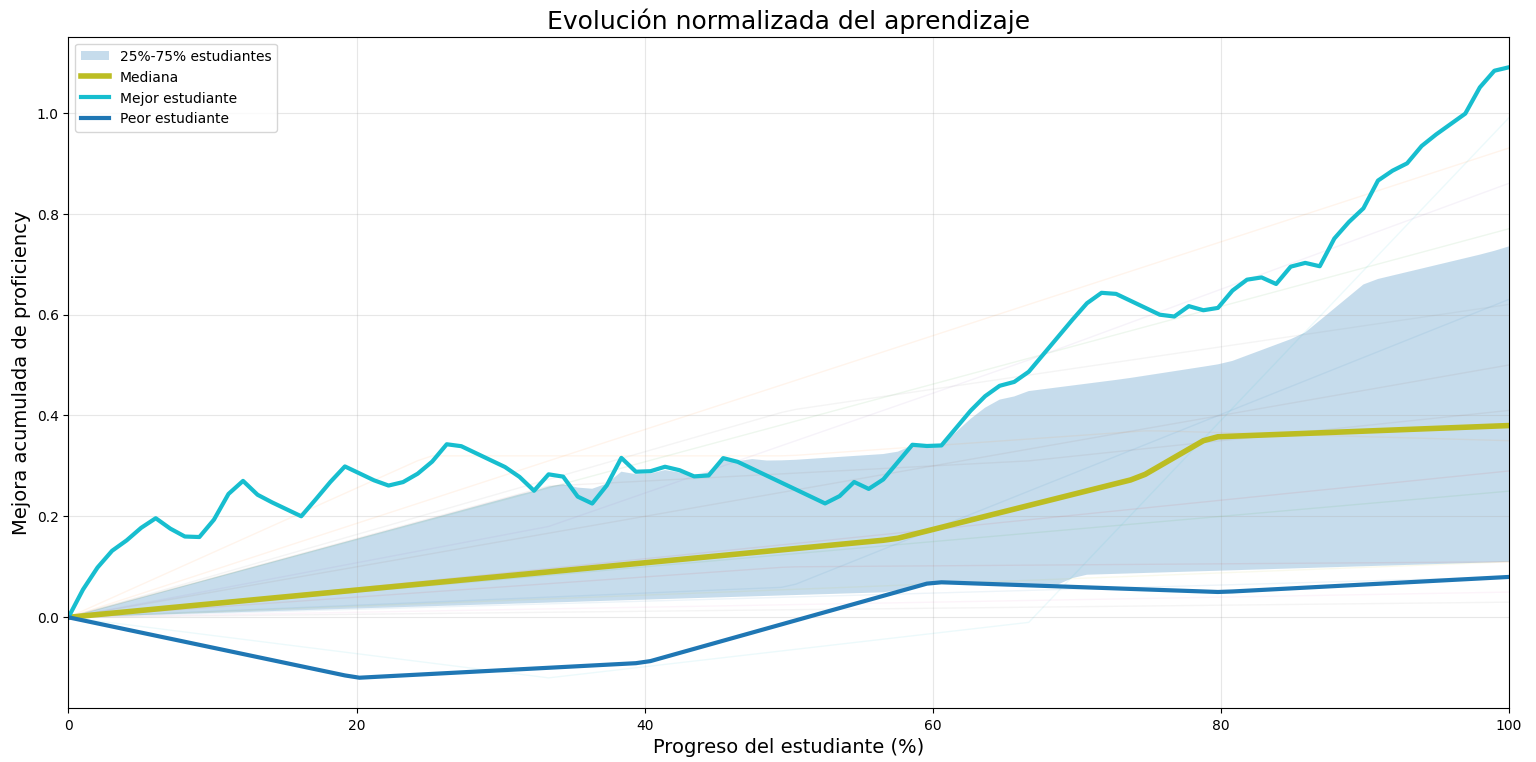
\includegraphics[width=0.48\textwidth]{Imagenes/rendimiento_estudiantes.png}
    \caption{Evolución del nivel de \textit{proficiency} de tres perfiles representativos de estudiantes durante la validación experimental.}
    \label{fig:rendimiento_ieee}
\end{figure}

La continuidad de uso fue evaluada mediante el número de sesiones registradas durante el período experimental. Como se observa en la Figura~\ref{fig:actividad_ieee}, la actividad se mantuvo estable durante las tres primeras semanas de evaluación, acumulando un total de 572 sesiones. La disminución observada durante la cuarta semana corresponde al cierre del proceso de recolección de datos y no a una disminución en el uso de la plataforma.

\begin{figure}[htbp]
    \centering
    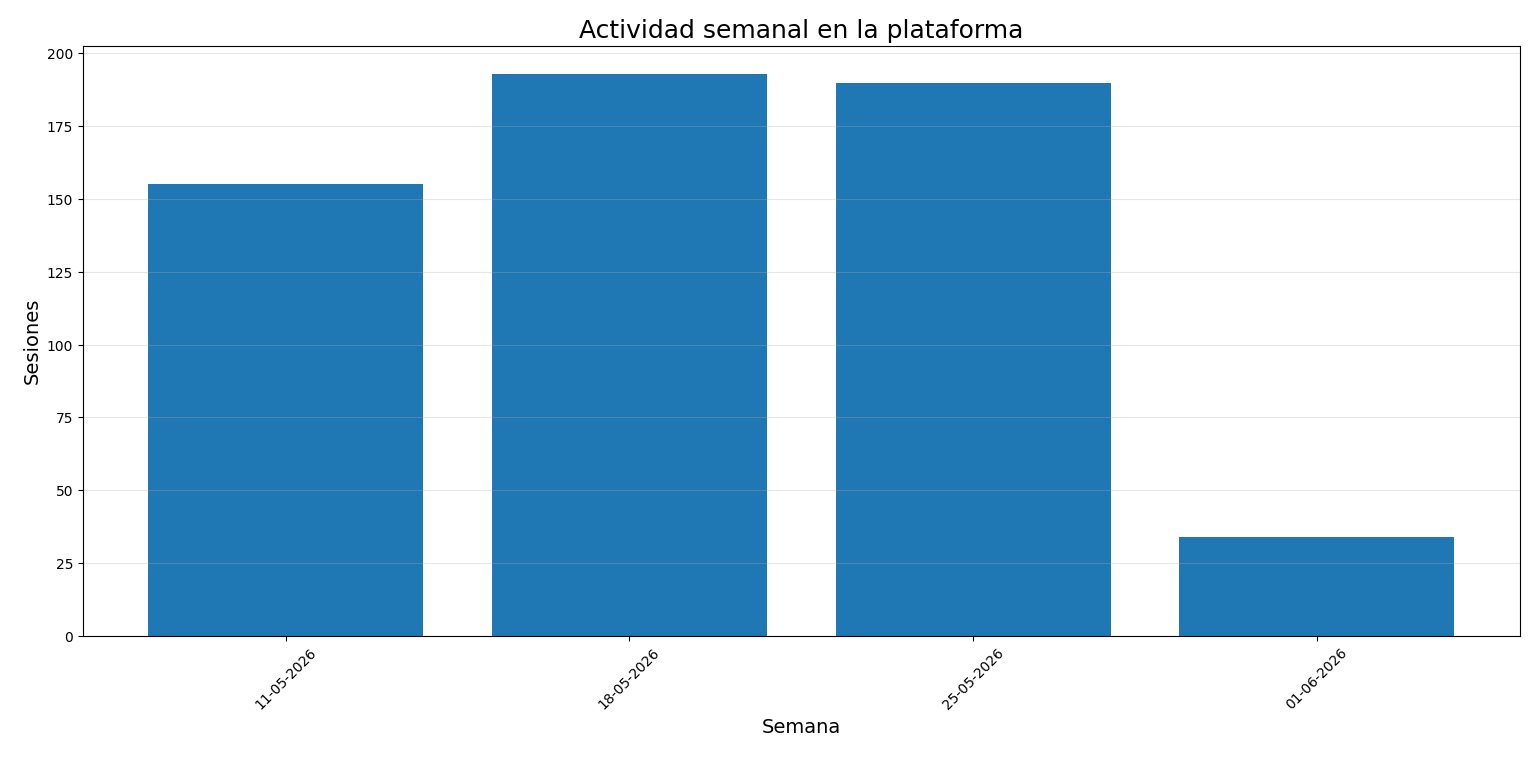
\includegraphics[width=0.48\textwidth]{Imagenes/actividad_semanal.png}
    \caption{Distribución semanal de las sesiones registradas durante el período de validación.}
    \label{fig:actividad_ieee}
\end{figure}

Los principales indicadores obtenidos durante la validación se resumen en la Tabla~\ref{tab:resultados_ieee}. En particular, la mediana del nivel de \textit{proficiency} presentó una mejora aproximada del 20\%, superando la meta inicial del 15\%. Asimismo, el sistema ajustó dinámicamente la dificultad y la secuencia de ejercicios de acuerdo con el desempeño individual de cada estudiante, evidenciando la capacidad del agente DRL para personalizar el proceso de aprendizaje.

\begin{table}[htbp]
\centering
\caption{Resumen de los principales resultados obtenidos durante la validación del modelo de recomendación.}
\label{tab:resultados_ieee}
\begin{tabular}{lp{5.2cm}}
\hline
\textbf{Indicador} & \textbf{Resultado} \\
\hline
Participantes & 28 estudiantes \\
Sesiones registradas & 572 sesiones \\
Continuidad de uso & Actividad sostenida durante el período de evaluación \\
Mejora en \textit{Proficiency} & Incremento aproximado del 20\% (meta: 15\%) \\
Adaptabilidad & Ajuste dinámico de la dificultad y secuencia de ejercicios según el desempeño del estudiante \\
\hline
\end{tabular}
\end{table}

En conjunto, estos resultados indican que el agente basado en \textit{Deep Reinforcement Learning} fue capaz de mantener una progresión positiva del aprendizaje, adaptar las recomendaciones al desempeño individual de los estudiantes y sostener una participación continua durante el período de evaluación.

%--------------------------------------------------------
\subsubsection{Resultados de la Plataforma}

La plataforma \textbf{SheetMusic} fue evaluada desde la perspectiva de la experiencia de usuario utilizando los instrumentos \textit{System Usability Scale} (SUS) y \textit{Technology Acceptance Model} (TAM). Los resultados obtenidos se resumen en la Tabla~\ref{tab:sus_tam}.

\begin{table}[htbp]
\centering
\caption{Resultados de la evaluación de usabilidad y aceptación tecnológica de la plataforma.}
\label{tab:sus_tam}
\begin{tabular}{lc}
\hline
\textbf{Métrica} & \textbf{Resultado} \\
\hline
System Usability Scale (SUS) & 82.5 / 100 \\
Future Use Perception (FUP) & 4.00 / 5.00 \\
\hline
\end{tabular}
\end{table}

El puntaje obtenido en SUS indica una percepción positiva respecto de la facilidad de uso de la plataforma, mientras que la evaluación de Future Use Perception evidencia una favorable disposición de los participantes a continuar utilizando la herramienta en futuros procesos de enseñanza y aprendizaje. En conjunto, estos resultados complementan la evaluación técnica del modelo de recomendación, mostrando que la propuesta no sólo adapta el proceso de aprendizaje, sino que además presenta un nivel de usabilidad y aceptación adecuado para su utilización en contextos educativos.